 % LuaLaTeX文書; 文字コーAドはUTF-8
 \documentclass[unicode,12pt, A4j]{ltjsarticle}% 'unicode'が必要
 %\usepackage{luatexja}% 日本語したい
 \usepackage{luatexja-fontspec}
 %\usepackage[hiragino-pron]{luatexja-preset}% IPAexフォントしたい(ipaex)
 \usepackage[hiragino-pron,deluxe,expert,bold]{luatexja-preset}

 \usepackage[english]{babel}%多言語文書を作成する
 \usepackage{amsmath,amssymb}%標準数式表現を拡大する
 \usepackage{physics}
 \usepackage[subpreambles=true,sort=true]{standalone}
% \renewcommand{\kanjifamilydefault}{\gtdefault}% 既定をゴシック体に
 %\usepackage[style=authoryear,backend=bibtex]{biblatex}
\usepackage{tikz}
\usetikzlibrary{arrows.meta}
\usetikzlibrary{calc}
 \usepackage{mhchem}
 % あとは欧文の場合と同じ

  \usepackage{caption}
  \usepackage[subrefformat=parens]{subcaption}

% https://mathlandscape.com/latex-style/
\everymath{\displaystyle}
\title{東大数学理科後期2002年度}
\author{}
\date{}

\begin{document}
\maketitle

\section{問題1}
実数全体で定義された関数$f(x) = xe^{-x^2}$を考える。

\begin{enumerate}
  \item $f(x)$の増減・凹凸を調べ$f(x)$のグラフの概形を図示せよ。
  \item 正の数$C$に対して$y=f(x)$と$x$軸、および$x = C$で囲まれた領域を$D_1$とする。$D_1$を$x$軸のまわりに回転させて得られる立体の体積を$V_1(C)$とおくとき
  \begin{align}
  \lim_{C \to \infty} V_1(C)
  \end{align}  
  を求めよ。
  \item $y = f(x)$の$x \geq 0$における最大値を$M$とするとき$y = f(x)$と$y$軸、および$y = M$で囲まれた領域を$D_2$とおく。$D_2$を$y$軸のまわりに回転させて得られる立体の体積$V_2$を求めよ。
\end{enumerate}


\section{問題2}
$xyz$ 空間において次のような3つの互いに合同な長方形 $L_1, L_2, L_3$ を考える。
\begin{itemize}
    \item $L_1$ は $xy$ 平面に含まれ、$P_1(a, b, 0)$, $Q_1(-a, b, 0)$, $R_1(-a, -b, 0)$, $S_1(a, -b, 0)$ を頂点とする。
    \item $L_2$ は $yz$ 平面に含まれ、$P_2(0, a, b)$, $Q_2(0, -a, b)$, $R_2(0, -a, -b)$, $S_2(0, a, -b)$ を頂点とする。
    \item $L_3$ は $zx$ 平面に含まれ、$P_3(b, 0, a)$, $Q_3(b, 0, -a)$, $R_3(-b, 0, -a)$, $S_3(-b, 0, a)$ を頂点とする。
\end{itemize}
ここで $a > b > 0$ とする。このとき次の間に答えよ。

\begin{enumerate}
    \item $\triangle P_1 P_2 P_3$ の面積、および $\triangle P_1 P_2 P_3$ と原点 $O$ との距離を求めよ。
    \item 四面体 $O P_1 P_2 P_3$ および四面体 $O P_1 S_2 P_3$ の体積をそれぞれ求めよ。
    \item $L_1, L_2, L_3$ の12頂点から3点を選び三角形をつくる。このとき $\triangle P_1 P_2 P_3$ または $\triangle P_1 P_2 S_2$ と合同な三角形が20個えられる。これらの三角形で囲まれる立体を $D$ とする。 $0 < \theta < \frac{\pi}{4}$ なる $\theta$ に対して
    \[
    a = \cos \theta, \quad b = \sin \theta
    \]
    とおくとき $D$ の体積 $V$ を $t = \tan \theta$ の関数 $V(t)$ として表せ。
    \item $0 < t < 1$ において $V(t)$ は最大値をとることを示し、そのときの $t$ の値を求めよ。
\end{enumerate}

\begin{figure}[h]
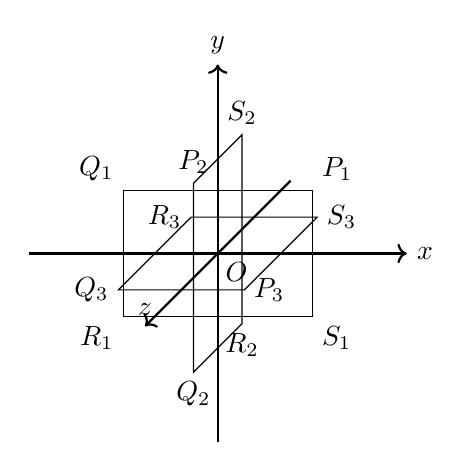
\begin{tikzpicture}[scale=0.8]
\draw[thick, ->] (-3,0) -- (3,0) node[right] {$x$};
\draw[thick, ->] (0,-3) -- (0,3) node[above] {$y$};
\draw[thick, ->] (0,0,-3) -- (0,0,3) node[above] {$z$};
\node at (0.3,-0.3,0) {$O$};

\draw (1.5,1,0) node[above right] {$P_1$} -- (-1.5,1,0) node[above left] {$Q_1$} -- (-1.5,-1,0) node[below left] {$R_1$} -- (1.5,-1,0) node[below right] {$S_1$} -- cycle;
\draw (0,1.5,1) node[above] {$P_2$} -- (0,-1.5,1) node[below] {$Q_2$} -- (0,-1.5,-1) node[below] {$R_2$} -- (0,1.5,-1) node[above] {$S_2$} -- cycle;
\draw (1,0,1.5) node[right] {$P_3$} -- (-1,0,1.5) node[left] {$Q_3$} -- (-1,0,-1.5) node[left] {$R_3$} -- (1,0,-1.5) node[right] {$S_3$} -- cycle;
\end{tikzpicture}       
\end{figure}




\section{問題3}
区間$[0,1]$において関数$f(x)$を
\begin{align}
f(x) =
\begin{cases}
2x & \left( x \leq \frac{1}{2} \right) \\
-2x + 2 & \left( x > \frac{1}{2} \right)
\end{cases}       
\end{align}
とおく。$0 \leq a_1 \leq 1$ を満たす実数 $a_1$ を初期値として数列 $\{a_n\}$ を
\begin{align}
a_n = f(a_{n-1}) \quad (n = 2, 3, \ldots)
\end{align}
で定める。このとき次の問に答えよ。

\begin{enumerate}
  \item $f(b) = b$ を満たす,$0 \leq b \leq 1$ なる実数をすべて求めよ。
  \item $a_4$ が (1) で求めたものの値の 1 つに等しくなるような初期値 $a_1$ をすべて求めよ。
  \item 条件
  \begin{quote}
    「ある $n \geq 1$ に対して、$a_n$ が (1) で求めたものの値の 1 つに等しくなる」
  \end{quote}
  を満たす初期値 $a_1$ はどのような実数として表されるか。
  \item 初期値 $a_1$ が (3) の条件を満たさないとき、$a_n = \frac{3}{4}$ となるような $n \geq 1$ が存在することを示せ。
  \item 数列 $\{a_n\}$ が収束するために初期値 $a_1$ が満たすべき必要十分条件を求めよ。
\end{enumerate}



\end{document}